\section{H-bro - Motorstyring}

Den bil der er fremskaffet til projektet er udstyret med en DC motor. For at styre hastighed, acceleration og deceleration skal forsyningen til DC motoren reguleres. En effektiv måde at gøre det på er med et PWM signal. Det gøres ved at ændre duty cycle på signalet som på figur \ref{fig:PWMpic}. For en mere uddybende forklaring på PWM konceptet se Wikipedia PWM \cite{lib:wikiPWM}
%\footnote{\url{https://en.wikipedia.org/wiki/Pulse-width_modulation}}

\begin{figure}[h]
	\centering
	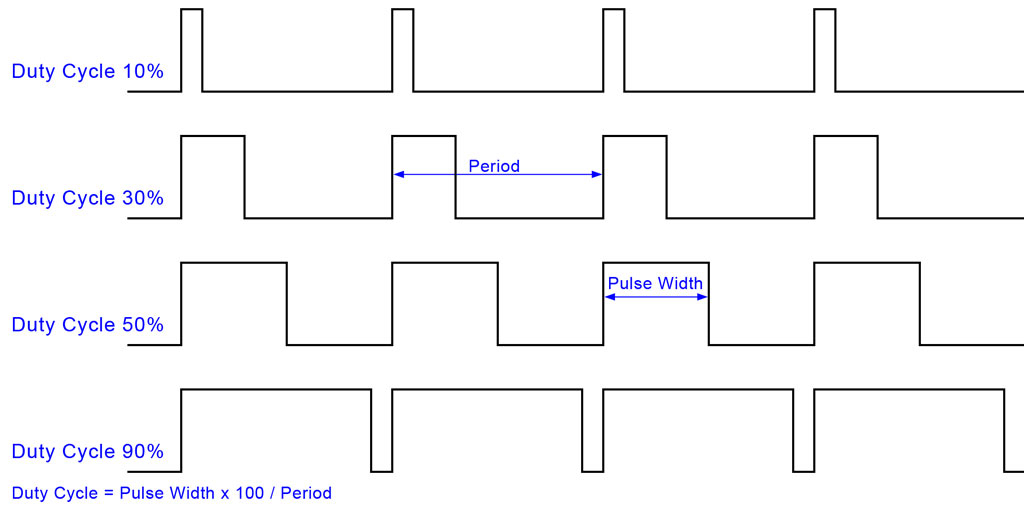
\includegraphics[width=\textwidth* 6/10]{../fig/billeder/pwm_lrg}
	\label{fig:PWMpic}
	\caption{Eksemple på PWM styring}
\end{figure}

Efter der i tidligere projekter er arbejdet med L298N\cite{lib:L298N_datablad}, som er en ''Dual Full Bridge Driver''/ Fuld H-bro, valgt til opgaven. H-broen virker som det ses på figur \ref{fig:H-bridge} ved at 2 kontakter sluttes for at kører den ene vej og de 2 andre for at kører den anden vej. Fordelen ved at bruge L298N er at ud over muligheden at sætte retning også er muligt at bruge et PWM signal på kontakterne. Og derved kan hastigheden reguleres.


\begin{figure}[ht]
	\centering
	\begin{minipage}[b]{0.29\linewidth}
		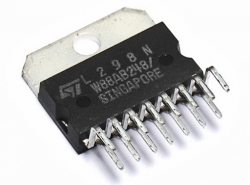
\includegraphics[width=\textwidth* 9/10]{../fig/billeder/L298N}
		\caption{L298N}
		\label{fig:L298N}
	\end{minipage}
	\quad
	\begin{minipage}[b]{0.68\linewidth}
		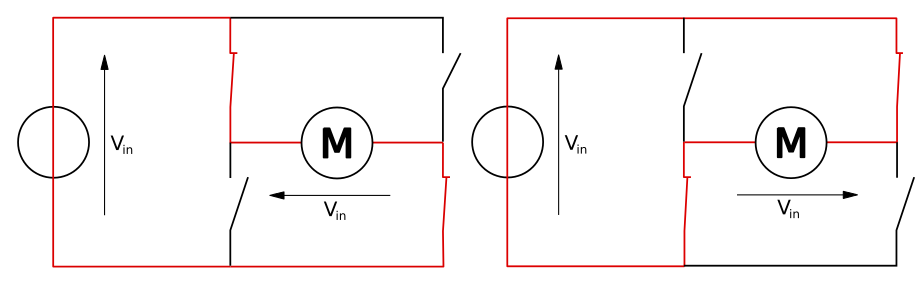
\includegraphics[width=\textwidth* 9/10]{../fig/billeder/H_bridge_operating}
		\caption{H-bridge princip fra Wikipedia \cite{lib:wikiHbro}}
		\label{fig:H-bridge}
	\end{minipage}
\end{figure}

L298N er internt opbygget som på figur \ref{fig:H_Bro_fra_L298N_datablad2}. Her ses det at In1 / In2 signalerne aktivere hvert deres sæt af mosfet's når Enable signalet aktiveres. Den øvre frekvens for hvor hurtig det er muligt at switche på denne H-bro er 40kHz. Vi vil vælge så høj en frekvens som muligt for at kommer over det hørbare område men samtidig så lavt at der ikke genererer generende EMC støj.

\clearpage
\begin{figure}[h]
	\centering
	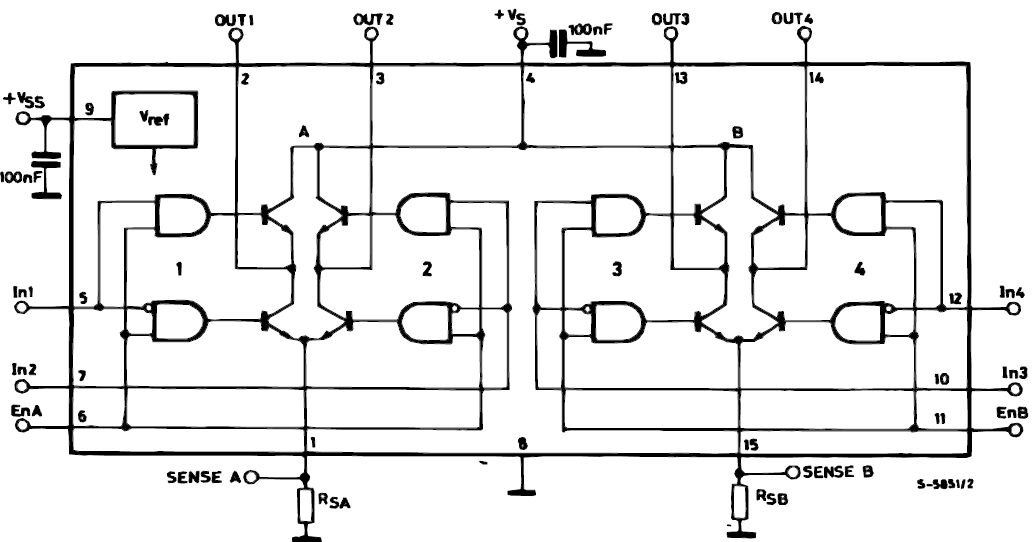
\includegraphics[width=\textwidth* 8/10]{../fig/billeder/L298N_data_2}
	\label{fig:H_Bro_fra_L298N_datablad2}
	\caption{Opbygning af H-Bro fra L298N's datablad \cite{lib:L298N_datablad}}
\end{figure}

\subsection*{MultiSim}

Kredsløbet til motorstyringen er designet i MultiSim efter anbefalingerne der er givet i databladet til L298N \cite{lib:L298N_datablad} samt tilføjet pulldown modstande på signalerne til enable, In1 og In2. For at være sikker på at signalerne ikke svæver og giver utilsigtede signaler til H-broen.
\begin{figure}[h]
	\centering
	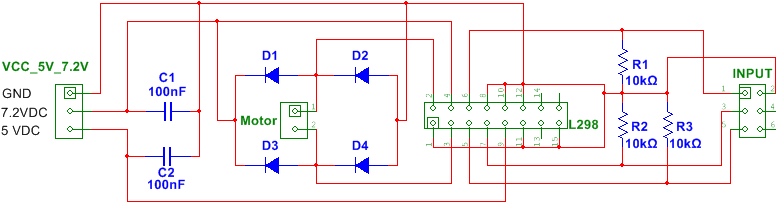
\includegraphics[width=\textwidth* 9/10]{../fig/billeder/MultiSim_H_Bro}
	\label{fig:MultiSim_HBro}
	\caption{MultiSim H-Bro}
\end{figure}





